\documentclass[12pt]{article}

% Essential packages
\usepackage[utf8]{inputenc}
\usepackage[T1]{fontenc}
\usepackage{lmodern}
\usepackage[english]{babel}

% Page layout - arXiv compliant (US letter, 1" margins)
\usepackage[letterpaper,margin=1in]{geometry}

% Spacing - single space for arXiv (comment out for double-space drafts)
% \usepackage{setspace}
% \doublespacing

% Math packages
\usepackage{amsmath}
\usepackage{amssymb}
\usepackage{amsthm}

% Graphics and figures
\usepackage{graphicx}
\usepackage{float}
\usepackage{tikz}
\usetikzlibrary{arrows.meta,positioning,calc}
\usepackage{caption}
\usepackage{subcaption}

% Tables
\usepackage{booktabs}
\usepackage{multirow}
\usepackage{array}
\usepackage{longtable}

% Links and references (hyperref should be loaded late)
\usepackage{xurl}
\usepackage{hyperref}
\hypersetup{
    colorlinks=true,
    linkcolor=blue,
    citecolor=blue,
    urlcolor=blue,
    pdfauthor={Anton Fedoruk, Serhii Shchoholiev, Akhil Mehta},
    pdftitle={LongListBench: A Benchmark for Long-List Entity Extraction from Complex Business PDFs},
    pdfsubject={Benchmark for long-list entity extraction from complex business PDFs},
    pdfkeywords={document understanding, information extraction, OCR, large language models, benchmark, long-list entity extraction, layout noise, multi-hop extraction},
    bookmarksnumbered=true,
    bookmarksopen=true,
    pdfstartview=FitH,
    pdfpagemode=UseOutlines,
}
\usepackage{cleveref}
\usepackage{orcidlink}  % ORCID iD icon + hyperlink

% Bibliography
\usepackage{csquotes}
\usepackage[style=ieee,sorting=none]{biblatex}
\addbibresource{references.bib}

% Custom theorem environments
\newtheorem{theorem}{Theorem}[section]
\newtheorem{lemma}[theorem]{Lemma}
\newtheorem{proposition}[theorem]{Proposition}
\newtheorem{corollary}[theorem]{Corollary}
\theoremstyle{definition}
\newtheorem{definition}[theorem]{Definition}
\newtheorem{example}[theorem]{Example}
\theoremstyle{remark}
\newtheorem{remark}[theorem]{Remark}

% Document metadata
\title{LongListBench: A Benchmark for Long-List Entity Extraction from Complex Business PDFs}
\author{
    Anton Fedoruk\textsuperscript{1}\thanks{\texttt{anton@kay.ai}}
    \hspace{2em}
    Serhii Shchoholiev\,\orcidlink{0009-0007-2014-4828}\textsuperscript{1}\thanks{\texttt{serhii@kay.ai}\quad\orcidlink{0009-0007-2014-4828}~\url{https://orcid.org/0009-0007-2014-4828}}
    \hspace{2em}
    Akhil Mehta\textsuperscript{1}\thanks{\texttt{akhil@kay.ai}}
    \\[1em]
    \normalsize\textsuperscript{1}Kay.ai, Brooklyn, NY, USA
}
\date{}

\begin{document}

\maketitle

\begin{abstract}
Current document extraction benchmarks focus on short, key-value forms, leaving long-list entity extraction, the recovery of hundreds or sometimes thousands of repeated records from tables and mixed layouts, underexplored. Business documents such as loss runs, invoices, and itemized bills commonly contain such lists. We introduce LongListBench, a synthetic benchmark for long-list extraction that pairs structured ground truth (JSON) with rendered documents and paired clean and OCR transcripts. This supports evaluation under complex layouts and OCR noise, while making OCR-specific degradation measurable without changing the underlying document.
The benchmark injects seven document phenomena observed in production (page breaks, multi-row entities, duplicates, large documents, distractor tables, multi-column layouts, and merged cells) to stress segmentation and schema-conformant extraction at scale. Using corpus-level field-value micro-averaging as the primary metric, a local full-context one-shot Gemini baseline on the OCR condition reaches 27.4\% $F_1$ overall and 5.9\% on the extreme tier, while a local auto-chunked Gemini baseline reaches 84.8\% overall and 81.7\% on the extreme tier. Chunking therefore substantially improves robustness on very long documents, but the simpler released baseline still leaves major residual errors, especially on long detailed documents, and should be viewed as a mitigation rather than a complete solution. We further evaluate a third, agentic regime in which GPT-5.5 is given only the OCR inside a code-execution sandbox and parses the document with its own tools rather than via fixed chunking; it reaches 90.6\% overall and 89.4\% on the extreme tier, the strongest result we observe, though as a more capable model it measures regime and model jointly.
%

\end{abstract}

\section{Introduction}
\label{sec:introduction}
Long-list entity extraction, the recovery of hundreds or sometimes thousands of repeated records from semi-structured documents, is a core requirement for document automation in domains such as insurance, finance, and procurement. While recent advances in document understanding models (e.g., layout-aware pretraining~\cite{xu2020layoutlm,huang2022layoutlmv3} and OCR-free approaches~\cite{kim2022donut}) and general-purpose LLMs have improved extraction quality, robust evaluation of long-list scenarios remains limited.

Many established benchmarks focus on key-value style extraction or relatively short, form-like documents (e.g., FUNSD~\cite{jaume2019funsd}) or narrow document types such as receipts (SROIE~\cite{huang2021sroie}, CORD~\cite{park2019cord}). Document question answering benchmarks such as DocVQA~\cite{mathew2021docvqa} and MP-DocVQA~\cite{tito2022mpdocvqa} highlight the additional difficulty of reasoning over document pages, especially in the multi-page setting. More recent datasets such as DocILE~\cite{simsa2023docile} include business documents and line items, but long lists in the wild often exhibit additional failure modes: repeated entities, page breaks, multi-column reading order, distractor tables, and table constructs such as merged cells. VRDU~\cite{wang2023vrdu} highlights that hierarchical and long-list fields remain challenging for LLM-based extraction.

We introduce LongListBench, a benchmark designed to stress-test long-list extraction from semi-structured business documents with long incident and line-item lists under systematically injected document phenomena. The benchmark is inspired by recurring patterns observed in real-world claims and policy-review documents. The core release is a controlled 80-document claims suite; we also include a 6-document single-PDF multi-hop extension for cases where target records must be assembled by joining fields across distant pages within the same PDF.

\subsection{Background and Motivation}
This work was motivated by production document-automation tasks involving long schedules, loss runs, and itemized bills. In these settings, a single document can contain hundreds or thousands of repeated entities spread across heterogeneous layouts, page breaks, and noisy OCR. Existing extraction systems often handled short forms adequately but degraded as list length and layout complexity increased. These observations motivated a benchmark that measures whether extraction methods remain reliable as list length grows and as layout artifacts accumulate.

\subsection{Research Questions}
This work is organized around four practical questions:
\begin{itemize}
    \item How do document format and tiered long-list stressors (page breaks, duplicates, multi-row entities, large documents, distractor tables, multi-column layouts, merged cells) affect extraction quality?
    \item To what extent are end-to-end failures attributable to OCR versus downstream extraction?
    \item How does a simple full-context one-shot baseline fail as documents grow longer and more complex?
    \item What benchmark structure is needed to evaluate contemporary agentic extraction systems, including cases that require long-range cross-page joins?
\end{itemize}


We address these questions by reporting baseline extraction performance by format and difficulty tier, releasing canonical transcripts plus reproducible OCR transcript generation for paired transcript-condition evaluation, shipping a standardized evaluation pipeline with saved predictions and regenerable reports, and adding a long-range cross-page multi-hop extension aimed at agentic extraction systems.

\subsection{Contributions}
We make the following contributions:
\begin{itemize}
    \item A reproducible benchmark generation pipeline that produces paired ground truth JSON, rendered HTML/PDF artifacts, canonical transcripts, and reproducible OCR transcript generation.
    \item A core suite of 80 documents (40 detailed, 40 table) containing 6{,}828 incident rows across four difficulty tiers, with an extreme tier reaching 500 incidents per document.
    \item A single-document cross-page multi-hop extension with 6 long PDFs: 3 claim-oriented cases with 77 target incidents and 3 commercial insurance policy cases with 345 target records across Businessowners Policy (BOP), Workers Compensation (WC), and Commercial General Liability (CGL) packets.
    \item A taxonomy of seven injected problem types and evaluation scripts for field-level scoring across clean and OCR transcripts.
    \item Baseline extraction artifacts that calibrate the task: one-shot prompting exposes severe long-document recall failures, while stronger protocols such as auto-chunking and an agentic code-execution sandbox illustrate why future work should evaluate the extraction protocol, not only the base model.
\end{itemize}


\section{Related Work}
\label{sec:related-work}
\input{contents/2_related_work}

\section{Benchmark Construction}
\label{sec:benchmark-construction}
LongListBench\footnote{Code, data, and implementation details are available at \url{https://github.com/kaydotai/longlistbench}.} is a synthetic benchmark for long-list entity extraction in semi-structured business documents with long incident and line-item lists, inspired by recurring patterns observed in real-world claims documents. Each benchmark instance consists of (i) structured ground-truth incidents in JSON, (ii) rendered HTML/PDF artifacts, and (iii) transcript conditions in Markdown.

\subsection{Entity schema}
Ground truth incidents follow a structured schema (see \hyperref[sec:appendix-schemas]{Appendix~A}) that includes incident identifiers, policy metadata, narrative text, and nested financial breakdowns (\texttt{bi}, \texttt{pd}, \texttt{lae}, \texttt{ded}). While downstream workflows often emphasize a small subset of high-value fields (e.g., incident identifiers, loss dates, and financial totals), our evaluator requires and scores the full schema.

\subsection{Document generation}
\Cref{fig:generation-pipeline} illustrates the benchmark construction pipeline, which consists of two phases.

\paragraph{Schema design (green path).}
Human annotators reviewed real insurance loss run documents from trucking companies to identify common fields, layouts, and formatting patterns. From this analysis, we defined a structured JSON schema capturing incident identifiers, policy metadata, narrative descriptions, and nested financial breakdowns. This schema serves as ground truth for evaluation.

\paragraph{Synthetic generation (purple path).}
 Rather than using real documents (which contain sensitive information), we generate synthetic documents that preserve realistic layout challenges:
 \begin{enumerate}
     \item \textbf{Problem configuration}: We identify recurring layout artifacts in real documents (e.g., page breaks splitting records, merged cells, and multi-column layouts) and encode them as configurable problem types.
     \item \textbf{Document rendering}: We generate synthetic incident records under the target schema, render them to HTML with selected problem types injected, and convert the resulting HTML to PDF via headless Chromium.
     \item \textbf{Canonical transcript}: We derive a clean transcript directly from the rendered HTML structure, preserving intended reading order, page boundaries, headers, tables, and distractor sections without OCR corruption.
     \item \textbf{OCR transcript}: We can obtain a noisy transcript for each PDF using Gemini OCR on rendered page images. OCR is regenerated after PDF changes rather than treated as a reusable static artifact.
     \item \textbf{Markdown output}: Canonical transcripts are stored as page-concatenated Markdown; OCR transcripts use the same layout after the OCR generation step.
 \end{enumerate}

\begin{figure}[ht]
    \centering
    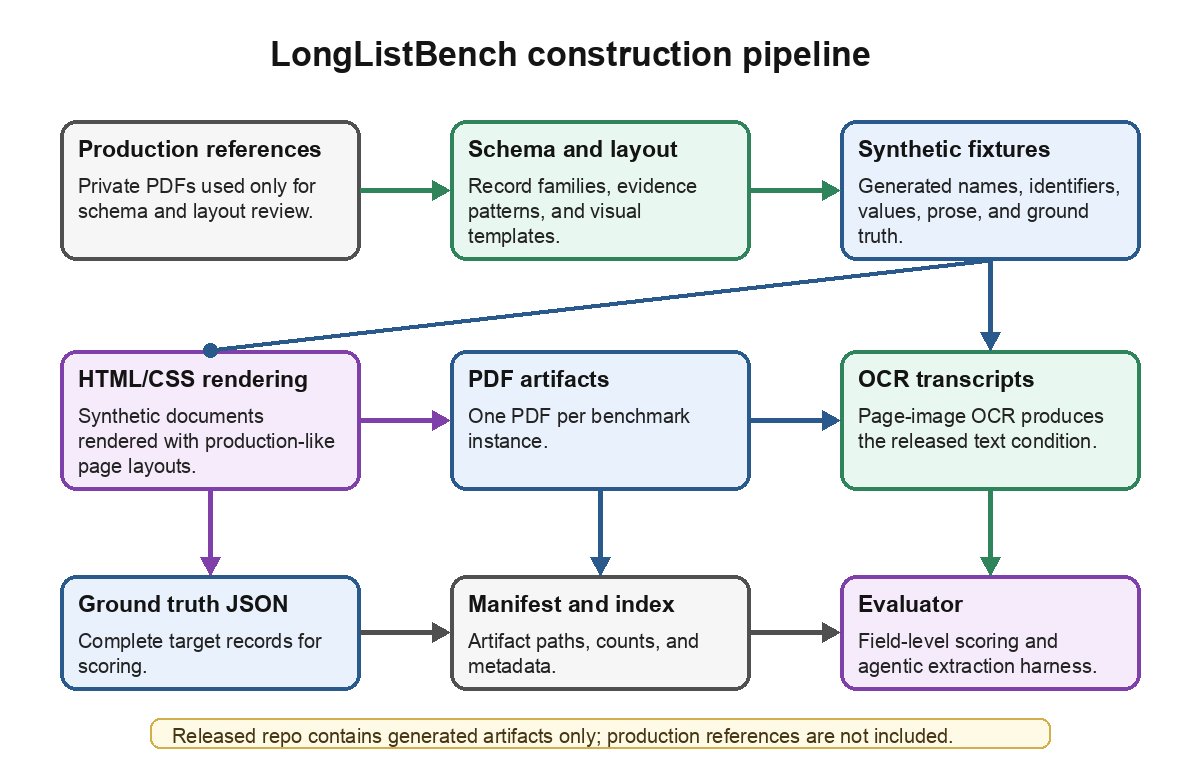
\includegraphics[width=0.7\linewidth]{figures/generation.png}
    \caption{Benchmark construction pipeline. Green path: schema design from real documents. Purple path: synthetic document generation and OCR processing.}
    \label{fig:generation-pipeline}
\end{figure}

Documents are rendered in one of two formats: (i) \textbf{Detailed}, which uses repeated incident blocks with narrative text and financial tables, or (ii) \textbf{Table}, which uses a compact tabular representation. The rendered PDFs also include synthetic packet covers, spreadsheet-like exports, portal receipts, request/response pages, and rotated scan excerpts inspired by recurring real-document layout patterns, without reusing private document content. All generation uses seeded randomness for reproducibility.

\subsection{Injected problem types}
We inject seven recurring document phenomena that complicate long-list extraction. These effects are applied at the HTML level prior to PDF rendering.

\paragraph{Page breaks.}
In real-world documents, page boundaries frequently interrupt local record context. In our detailed format, a single incident can begin on one page with identifiers and description while its financial breakdown appears on the next. In our table format, we instead insert page breaks between groups of rows and repeat table headers across the break. OCR systems typically process pages independently, producing separate text blocks that must be reassembled. Extraction models must therefore preserve continuity across pages and avoid dropping rows or misattaching continuation content.
\begin{figure}[ht]
    \centering
    \IfFileExists{figures/example_page_breaks.png}{
        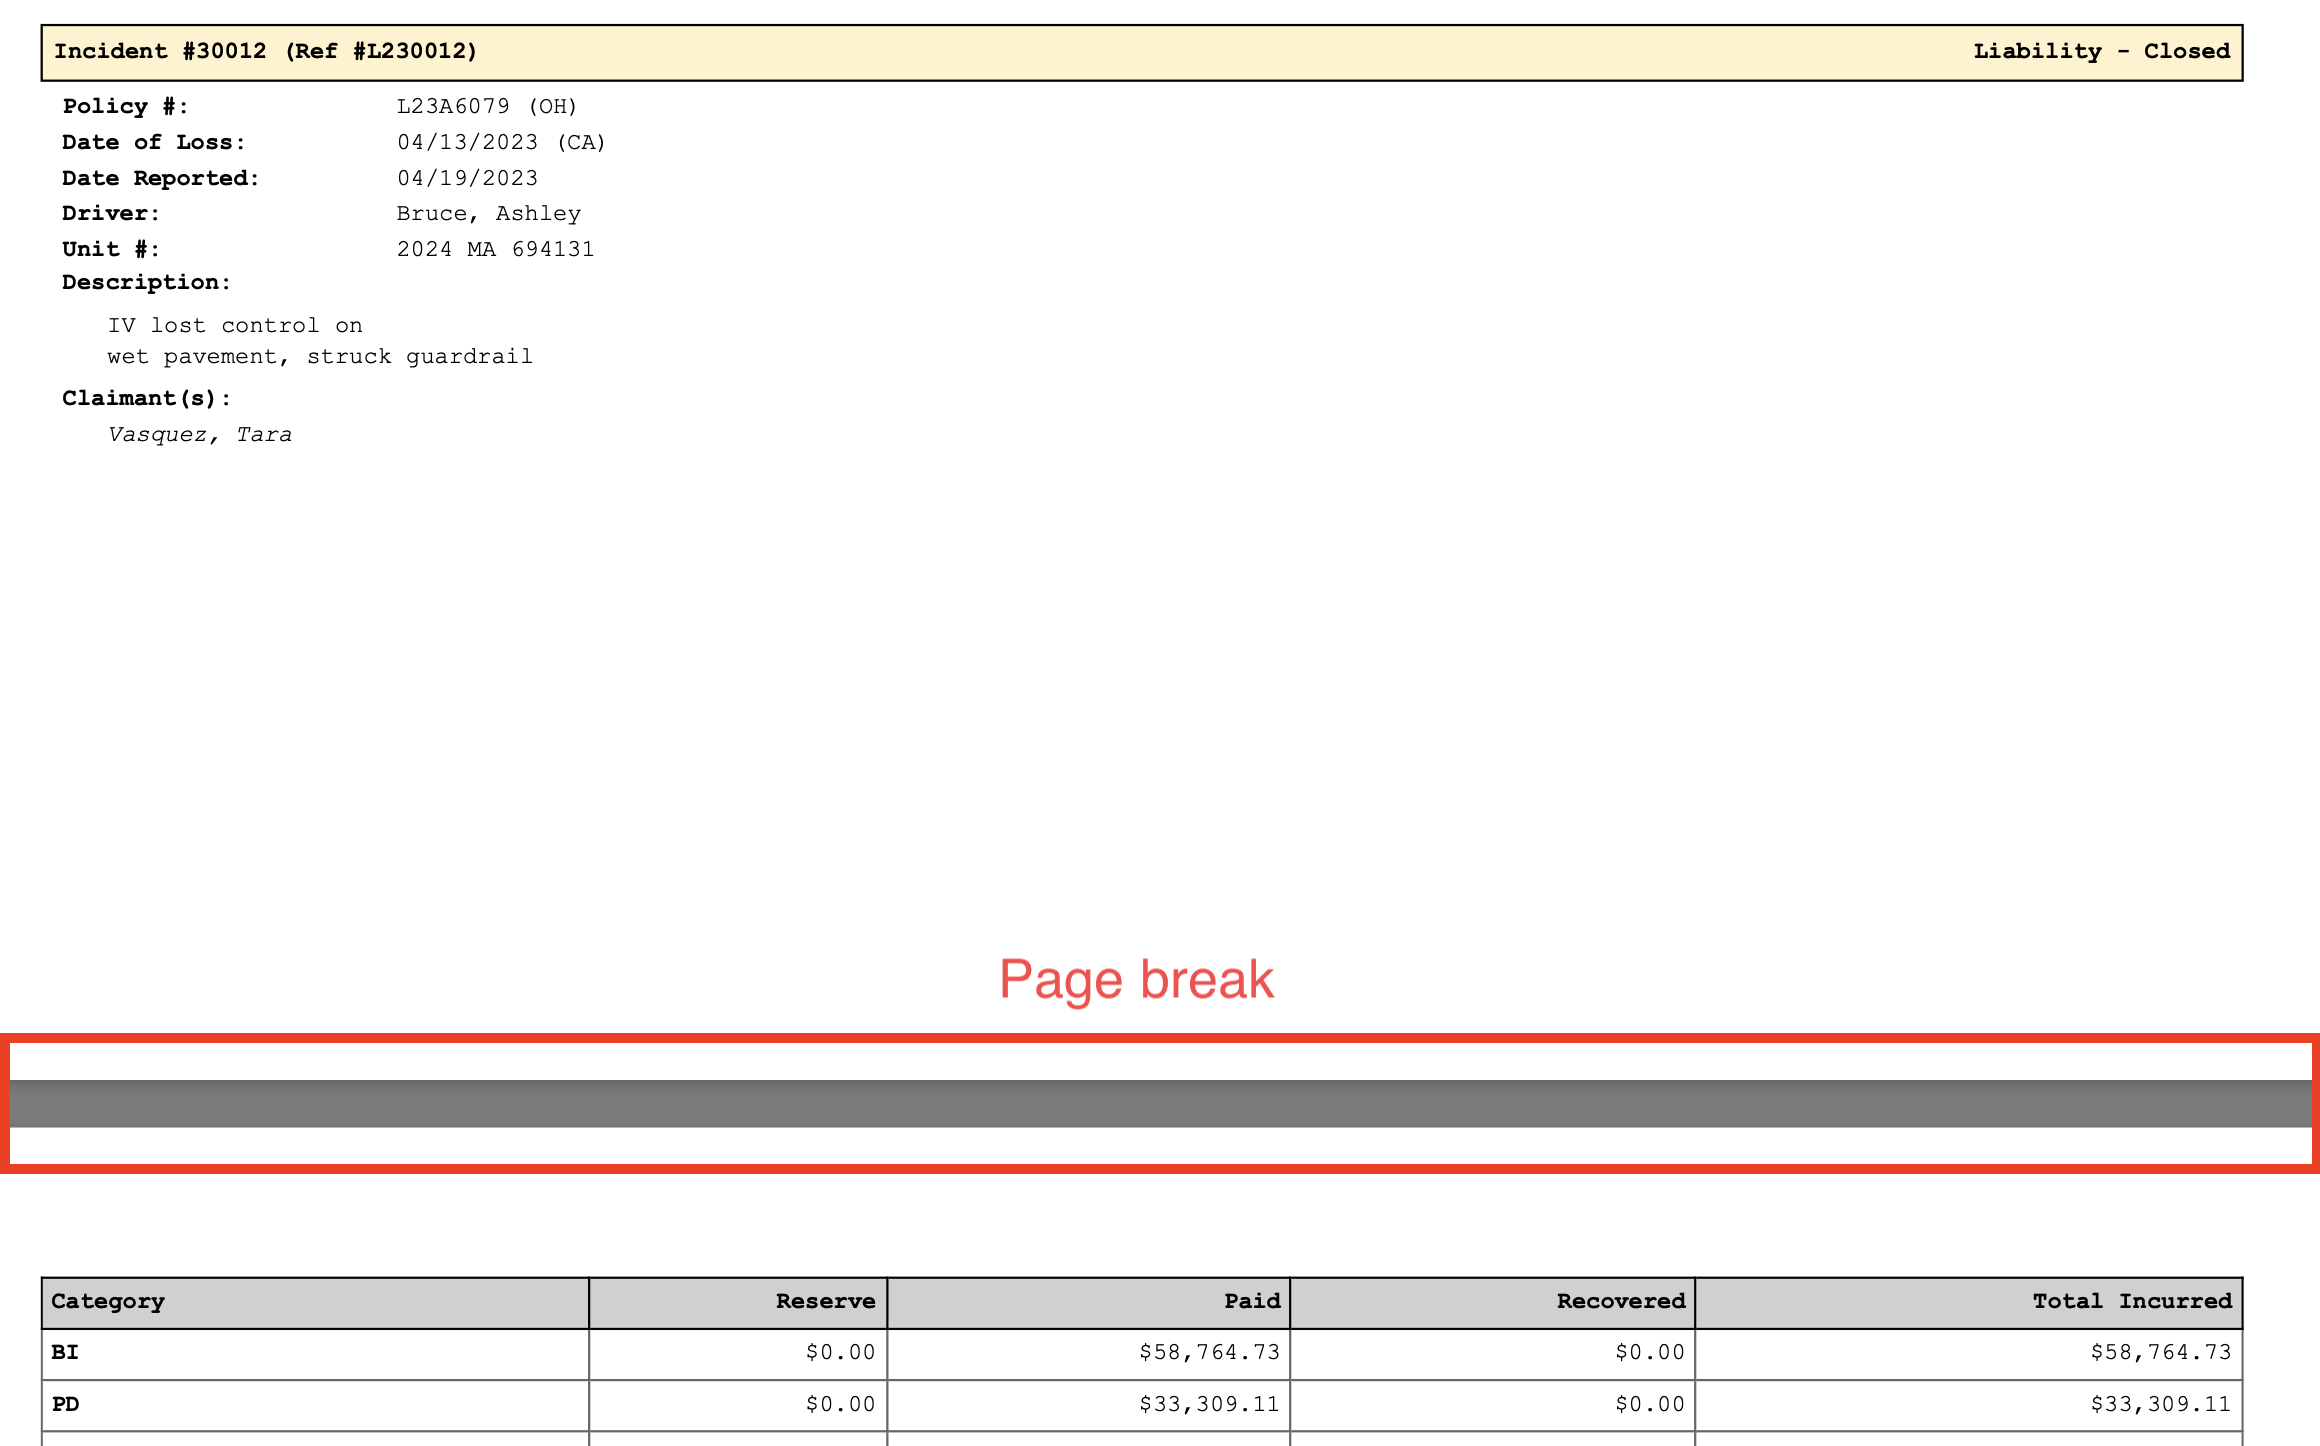
\includegraphics[width=0.95\linewidth]{figures/example_page_breaks.png}
    }{
        \fbox{\parbox{0.6\textwidth}{\centering\vspace{2cm}Page Breaks Example\vspace{2cm}}}
    }
    \caption{Example of an incident split across a page boundary.}
    \label{fig:example-page-breaks}
\end{figure}

\paragraph{Multi-row entities.}
Table cells often contain text that wraps across multiple lines, especially for description fields, addresses, or claimant lists. When OCR linearizes such content, it may interleave text from adjacent columns or treat each line as a separate cell. For example, a description spanning three lines might appear as three distinct rows in the OCR output, with column alignment lost. Extraction models must recognize that these lines belong to a single logical cell and reconstruct the original cell boundaries from visual or positional cues.
\begin{figure}[ht]
    \centering
    \IfFileExists{figures/example_multi_row.png}{
        \includegraphics[width=0.95\linewidth]{figures/example_multi_row.png}
    }{
        \fbox{\parbox{0.6\textwidth}{\centering\vspace{2cm}Multi-row Entities Example\vspace{2cm}}}
    }
    \caption{Example of a cell containing multiple lines of text.}
    \label{fig:example-multi-row}
\end{figure}

\paragraph{Exact duplicates.}
\mbox{}\\
Production documents sometimes contain intentionally repeated records. In insurance contexts, the same incident may appear multiple times due to amendments, re-openings, or reporting across multiple policy periods. Unlike data entry errors, these duplicates are semantically meaningful and must be preserved in the extracted output. Many extraction pipelines include deduplication as a post-processing step, which would incorrectly collapse valid duplicate entries. In LongListBench v1 we model this stressor as exact record repeats rather than near-duplicates or amended variants.

\paragraph{Large documents.}
Real loss runs and itemized bills routinely contain hundreds of line items. A single trucking company's annual loss run may list 200--500 incidents; a hospital bill for a complex procedure can exceed 1{,}000 charge lines. These documents push against context window limits of current LLMs. Even models with 128K+ token windows may exhibit degraded recall on items appearing in the middle of very long documents (the "lost in the middle" phenomenon). We include an extreme tier with 500 incidents per document to measure how extraction quality scales with document length.

\paragraph{Multiple tables.}
Business documents frequently embed auxiliary tables alongside the primary data. A loss run PDF might include a cover page with agent contact information, a summary table of totals by coverage type, or a glossary of status codes; none of these should be extracted as incident records. Models must distinguish the target entity table from these distractors based on schema matching, header recognition, or positional cues. Naive approaches that extract all tabular content will produce false positives from irrelevant tables.

\paragraph{Multi-column layout.}
Some documents use multi-column layouts to fit more content per page. This creates reading-order ambiguity: should text be read left-to-right across columns or top-to-bottom within each column? Standard OCR often assumes a single-column flow, interleaving content from parallel columns into an incoherent sequence. In LongListBench v1 this stressor primarily affects detailed-format primary content and auxiliary sections; the main table-format claims table remains single-span to preserve a readable tabular baseline.
\begin{figure}[ht]
    \centering
    \IfFileExists{figures/example_multi_column.png}{
        \includegraphics[width=0.95\linewidth]{figures/example_multi_column.png}
    }{
        \fbox{\parbox{0.6\textwidth}{\centering\vspace{2cm}Multi-column Layout Example\vspace{2cm}}}
    }
    \caption{Example of a two-column document layout.}
    \label{fig:example-multi-column}
\end{figure}

\paragraph{Merged cells.}
Tables often use merged cells for visual grouping. A common pattern is merging the company name cell across all incidents belonging to that company, or merging a coverage type header across its associated rows. In the rendered PDF, these appear as single cells spanning multiple rows or columns. OCR may report the merged cell's content only once, leaving subsequent rows with empty values for that field. Extraction models must propagate the merged value to all spanned rows, recognizing that an empty cell indicates inheritance from above rather than a missing value.
\begin{figure}[ht]
    \centering
    \IfFileExists{figures/example_merged_cells.png}{
        \includegraphics[width=0.95\linewidth]{figures/example_merged_cells.png}
    }{
        \fbox{\parbox{0.6\textwidth}{\centering\vspace{2cm}Merged Cells Example\vspace{2cm}}}
    }
    \caption{Example of a table with merged and spanning cells.}
    \label{fig:example-merged-cells}
\end{figure}

\subsection{Dataset scale}
The core released suite (\texttt{longlistbench-v1}, version 1.0.2) contains 80 rendered documents (40 detailed, 40 table) with 6{,}828 incident rows and canonical transcripts for evaluation. Difficulty tiers are configured as 15 easy base instances (seeded with 10 claims/PDF), 12 medium (25), 8 hard (50), and 5 extreme instances seeded with 100 claims/PDF and then expanded to 500 incidents per released document via \texttt{large\_doc}. Each base instance is rendered in both detailed and table formats, yielding 80 documents in total. Enabling \texttt{duplicates} injects additional duplicate rows, causing some documents to exceed the seed count. OCR transcripts can be generated from the rendered PDFs and should be regenerated whenever PDFs are changed.

Across the 80 documents, the most common injected issues are multi-row entities (62/80), page breaks (56/80), duplicates (56/80), and multiple tables (40/80).

\subsection{Long-range cross-page multi-hop extension}
Many production extraction tasks are not contained in one adjacent table region. A target loss-run record may require joining a front-matter claim schedule against policy registers, driver rosters, cause-code appendices, claimant indexes, and payment ledgers that appear much later in the same PDF. This pattern is awkward for one-shot extraction and naive chunking because the model must preserve join keys across large page and token distances, then merge partial records without confusing distractor rows.

To make this failure mode measurable, we add an initial multi-hop extension in the shared \path{data/} layout. It currently contains 6 single-document cross-page PDFs. Three claim-oriented cases contain 77 target incidents and use the same incident schema as the core suite; the rendered PDFs are 76, 126, and 198 pages. Three additional cases are synthetic commercial insurance policy packets: Businessowners Policy (BOP), Workers Compensation (WC), and Commercial General Liability (CGL). A policy packet is the contract document issued by an insurer; it combines declarations, covered locations or classifications, coverage limits and deductibles, rating or premium schedules, required forms, and endorsements that modify the base policy. These policy cases contain 345 target records across heterogeneous schemas for locations, coverage items, class-code or exposure items, forms, endorsements, and premiums. Each case includes one PDF, one HTML source, one \path{ground_truth} JSON file, a canonical transcript, reproducible OCR transcript generation, and per-sample metadata describing the evidence map and join requirements.

The claim-oriented extension uses the following join patterns:
\begin{itemize}
    \item \texttt{policy\_number} $\rightarrow$ policy register for company, insured, division, policy state, and agency fields.
    \item \texttt{unit\_number} $\rightarrow$ driver roster for driver identity.
    \item \texttt{cause\_code} $\rightarrow$ cause-code appendix for coverage type and normalized description.
    \item \texttt{incident\_number} $\rightarrow$ claimant index and financial ledger for claimants, adjuster notes, and nested financial breakdowns.
\end{itemize}

The policy-oriented extension adds joins such as location/building numbers to described premises, form numbers to forms-and-endorsements schedules, class codes to rating schedules, and coverage or endorsement references to distant detail pages. The largest cross-page documents mix these joins with archived distractor sections that reuse overlapping policy/reference values but contain out-of-scope records. This design is intended to stress extraction systems that can inspect long documents, preserve join keys across distant sections, and verify record completeness. The claim-oriented cases preserve comparability with the base incident schema and scorer; the policy-oriented cases use the heterogeneous record-list scorer released with the evaluation pipeline.


\section{Evaluation}
\label{sec:evaluation}
We evaluate systems on the task of extracting a complete list of target records from each rendered PDF or from its OCR transcript. Each sample is evaluated as a new document: the extractor receives the document input and the target schema or field contract, then returns all records for that document. A valid prediction is a JSON object whose top-level list is \texttt{incidents} for claim multi-hop incident tasks and \texttt{records} for operations, external loss-run, and policy list tasks.

\subsection{Input condition}
The current release includes an OCR transcript for every PDF. The evaluator treats the transcript condition as part of the experiment configuration, so future runs can compare OCR transcripts, direct PDF inputs, or additional OCR engines without changing the ground truth. Results should therefore report the input condition, model, extraction protocol, and whether the run includes long-range multi-hop samples.

\subsection{Extraction protocols}
LongListBench is designed to compare extraction protocols, not only base models. The evaluator scripts support prompt-based extraction and an agentic sandbox protocol.

\paragraph{Full-context one-shot extraction.}
The entire selected transcript is provided to the model in a single call. This regime is intentionally simple and is expected to fail on long documents when the model truncates, omits middle records, merges rows, or cannot maintain the full schema across thousands of fields. It is useful as a lower-bound calibration.

\paragraph{Agentic sandbox extraction.}
The agentic regime places the OCR transcript inside a sandbox and gives the model filesystem and code-execution tools. The model receives the target schema or field contract, decides how to inspect and segment the document, writes a JSON output file, and can run verification code before finishing. This protocol is a better match for long-list and long-range evidence tasks because it can search, slice, parse tables, and verify counts programmatically.

\paragraph{Parser and template diagnostics.}
Template-specific parsers are useful sanity checks, especially for structured operations families, but they are not the central benchmark target. In realistic agentic extraction, the system is given the current document and may write document-specific code if that is the most reliable way to recover the records. A parser trained on one template and frozen for another answers a different question: template-transfer robustness. We therefore treat deterministic parsers as diagnostics for identifying control families and parser-friendly layouts, while primary comparisons should use per-document extraction protocols run under the same input condition.

\paragraph{Other protocols.}
The evaluator scripts can also support fixed chunking, retrieval loops, and verification passes. These are extraction protocols and should be reported explicitly, because protocol design can dominate performance on long documents.

\subsection{Regime-aware reporting}
Aggregate micro-$F_1$ is useful, but it can hide which document complexities matter. We recommend reporting results by release config and by stressor metadata. The core operations config contains scale and completeness controls, including IFTA and spreadsheet-like reports where table extraction can be nearly deterministic. The claim and policy packet configs are the primary hard regimes: they require inherited context, distant evidence, heterogeneous schemas, and distractor handling inside one document. A strong result report should therefore include at least: corpus micro-$F_1$, document-macro summaries, predicted record counts, per-config scores, and stressor slices for \path{ocr_layout_condition}, \path{cross_section_join}, \path{long_range_evidence}, and \path{heterogeneous_record_list}.

\subsection{Validation and report regeneration}
Model outputs are parsed, normalized, and scored against the per-document ground truth. Reports are stored as machine-readable JSON with Markdown summaries. The checker can regenerate metrics from saved predictions and golden data, which makes it possible to audit reports without rerunning model calls.

\subsection{Field-level matching and metrics}
The primary metric is corpus-level micro precision/recall/$F_1$ over flattened field-value pairs. This weighting reflects the benchmark's purpose: a 2{,}000-row document should contribute more evidence than a 50-row document.

For claim incidents, records are keyed by normalized incident identifiers. Dates are normalized to \texttt{MM/DD/YYYY}, claimant lists are sorted, zero-valued default financial-breakdown cells are not scored, and non-zero monetary fields are rounded to cents before scoring. For generic record lists, records are matched greedily by overlapping non-global field pairs; \texttt{record\_type} and hidden row identifiers are not required for matching or scoring.

Let $G$ be the multiset of flattened field-value pairs from the ground truth and $P$ the multiset from predictions after canonicalization. We compute:
\begin{align}
\mathrm{found} &= |G \cap P|,\\
\mathrm{recall} &= \frac{\mathrm{found}}{|G|},\\
\mathrm{precision} &= \frac{\mathrm{found}}{|P|},\\
\mathrm{F1} &= \frac{2\,\mathrm{precision}\,\mathrm{recall}}{\mathrm{precision}+\mathrm{recall}}.
\end{align}
Reports also include predicted record counts, missing and extra record diagnostics, exact-record matches where meaningful, and per-document summaries.


\section{Results}
\label{sec:results}
This revision reports corpus validation and four OCR-conditioned agentic extraction baselines on the released corpus of 32 documents. Earlier prerelease experiments used a development set of 80 documents with different templates, schemas, and scoring. We retain those experiments as development history but do not mix their scores with the current release.

\subsection{Artifact completeness}
Each manifest instance has one PDF, HTML source, JSON ground-truth file, metadata file, and OCR transcript. The release contains 28{,}255 non-policy records and 1{,}344 policy records, for 29{,}599 targets overall. \Cref{tab:release-validation} summarizes the release gates.

\begin{table}[H]
\centering
\small
\caption{Current release validation summary.}
\label{tab:release-validation}
\begin{tabular}{@{}lr@{}}
\toprule
Check & Value \\
\midrule
Manifest instances & 32 \\
PDF, HTML, ground-truth, metadata, and OCR artifacts & 32 each \\
Total target records & 29{,}599 \\
Released transcript condition & OCR \\
Average identifier coverage & 99.9\% \\
Tracked identifier-field support & 99.9\% \\
Records with missing tracked OCR identifiers & 17 \\
Audited numeric OCR misses & 56 of 76{,}968 (0.073\%) \\
\bottomrule
\end{tabular}
\end{table}

The largest scale family, mileage by vehicle, contributes 17{,}565 records across eight PDFs. Structural families add sparse enrichment, split schedules, mixed row/detail blocks, heterogeneous records, and evidence distributed across sections. All 32 OCR transcripts pass the 95\% identifier-coverage gate. A numeric audit records 56 genuine OCR misses among 76{,}968 checked ground-truth numeric fields with absolute value at least 10. The transcripts are not hand-corrected, and the exact miss set is released. These checks bound the OCR condition; they are not extraction scores.

\subsection{Agentic OCR baselines}
\label{subsec:current-ocr-baseline}
Each run received one OCR transcript and the public field contract in a temporary workspace. A macOS sandbox denied the benchmark repository, and ground truth, target values and counts, and generator code were absent. Agents could inspect the transcript, write temporary code, validate JSON, and return the complete list. These are protocol baselines, not raw one-shot model measurements.

All four full-corpus runs were produced on July 14, 2026 at xhigh effort using Codex CLI 0.144.4 or Claude Code 2.1.209. Claude Code safe mode disabled project instructions, skills, plugins, hooks, and MCP servers. Per-sample metadata confirms the requested primary model in every run and records any auxiliary routing. All reports cover the same 29{,}599-target manifest with zero execution errors, and saved predictions reproduce every score in \Cref{tab:agentic-full-corpus}.

\begin{table}[H]
\centering
\footnotesize
\caption{Full-corpus agentic OCR baselines. Strict completeness is primary; field $F_1$ is secondary partial credit.}
\label{tab:agentic-full-corpus}
\begin{tabular}{@{}p{0.31\linewidth}rrrr@{}}
\toprule
Agent and model & Exact recall & Complete docs & Micro-$F_1$ & Macro-$F_1$ \\
\midrule
Codex CLI, GPT-5.6-Sol (xhigh) & 93.7\% & 6/32 (18.8\%) & 98.7\% & 98.3\% \\
Claude Code, Fable 5 (xhigh) & 90.9\% & 6/32 (18.8\%) & 96.1\% & 92.6\% \\
Codex CLI, GPT-5.5 (xhigh) & 90.4\% & 4/32 (12.5\%) & 98.2\% & 97.7\% \\
Claude Code, Opus 4.8 (xhigh) & 93.6\% & 7/32 (21.9\%) & 98.8\% & 98.4\% \\
\bottomrule
\end{tabular}
\end{table}

No configuration completes more than 7 of 32 documents. GPT-5.6-Sol has the highest exact-record recall, while Opus 4.8 completes one more document and has the highest field $F_1$. The family results below are more informative than this narrow aggregate ranking.

We preassign four parser-friendly families as scale controls and the other seven as structural challenges. \Cref{tab:agentic-by-role} reports the latest models by role.

\begin{table}[H]
\centering
\scriptsize
\caption{Strict completeness by evaluation role for the latest models.}
\label{tab:agentic-by-role}
\begin{tabular}{@{}p{0.24\linewidth}rrrrrr@{}}
\toprule
Role & Docs & Records & Sol exact & Fable exact & Sol complete & Fable complete \\
\midrule
Structural challenges & 19 & 8{,}414 & 79.0\% & 69.3\% & 2/19 (10.5\%) & 2/19 (10.5\%) \\
Scale controls & 13 & 21{,}185 & 99.5\% & 99.5\% & 4/13 (30.8\%) & 4/13 (30.8\%) \\
\bottomrule
\end{tabular}
\end{table}

\Cref{tab:agentic-by-regime} uses problem-first labels so the extraction challenge is visible without domain knowledge. Labels map one-to-one to the public \texttt{complexity\_regime} values.

\begin{table}[H]
\centering
\scriptsize
\caption{Latest-model exact-record recall by extraction problem. The divider separates structural challenges from scale controls.}
\label{tab:agentic-by-regime}
\begin{tabular}{@{}p{0.47\linewidth}rrrr@{}}
\toprule
Extraction problem & Docs & Records & GPT-5.6-Sol & Fable 5 \\
\midrule
Sparse record enrichment (driver/MVR) & 3 & 1{,}260 & 0.6\% & 1.9\% \\
Long-range claim joins & 3 & 77 & 98.7\% & 98.7\% \\
Split return schedules & 3 & 2{,}737 & 95.5\% & 95.5\% \\
Mixed row/detail loss runs & 3 & 900 & 97.3\% & 92.2\% \\
Tax inquiry detail tables & 2 & 1{,}300 & 99.9\% & 99.8\% \\
Heterogeneous policy records & 3 & 1{,}344 & 73.3\% & 14.6\% \\
Cross-section return joins & 2 & 796 & 99.6\% & 99.6\% \\
\midrule
Tax-summary scale controls & 2 & 1{,}520 & 99.5\% & 99.5\% \\
Driver-schedule scale control & 1 & 500 & 99.8\% & 99.8\% \\
Mileage-by-vehicle scale controls & 8 & 17{,}565 & 99.4\% & 99.4\% \\
Vehicle-schedule scale controls & 2 & 1{,}600 & 100.0\% & 100.0\% \\
\bottomrule
\end{tabular}
\end{table}

The failures differ in kind. GPT-5.6-Sol returns 1{,}259 driver rows but only 8 are exact; Fable 5 returns 1{,}243 and matches 24 exactly. Their driver/MVR field $F_1$ remains 88.0\% and 88.4\%, showing that most roster fields are present while sparse enrichment fields are not joined correctly. Both systems match 2{,}614 of 2{,}737 split-schedule records and 76 of 77 long-range claim records. Policy packets separate them: GPT-5.6-Sol matches 985 of 1{,}344 records with 95.8\% field $F_1$, while Fable 5 returns only 232 records, matches 196, and reaches 33.5\% field $F_1$. Scale controls remain near ceiling, yet only four of 13 are completely correct for either system because a single missing, extra, or malformed record fails document completion.

Cross-cutting slices reinforce this variation. Exact-record recall for GPT-5.6-Sol and Fable 5 is 73.3\% and 14.6\% on heterogeneous lists, 74.7\% and 19.1\% on long-range evidence, 94.9\% and 86.9\% on split records, 95.0\% and 87.0\% with inherited context, and 98.3\% and 98.3\% under layout randomization. Duplicate-bearing documents score 93.1\% and 73.4\%; cross-section joins and repeated keys score 99.6\% for both. These are observational associations because tags overlap and document families differ; paired renderings would be needed to estimate one stressor's causal effect.

Full-context one-shot extraction is not a practical full-corpus protocol here. Small claim packets can return scoreable outputs, but larger outputs reach model limits or time out. We therefore treat one-shot prompting as a lower-bound operational stress test and use the per-document agentic protocol for full-corpus comparison.


\section{Limitations and Intended Use}
\label{sec:limitations}
LongListBench is a measurement tool for long-list extraction under controlled synthetic conditions. Table~\ref{tab:benchmark-scope} summarizes the current scope.

\begin{table}[t]
\centering
\caption{Scope of the current LongListBench release.}
\label{tab:benchmark-scope}
\begin{tabular}{>{\raggedright\arraybackslash}p{0.46\linewidth} >{\raggedright\arraybackslash}p{0.46\linewidth}}
\toprule
Covered & Not covered / out of scope \\
\midrule
High-density insurance and trucking-operation lists, claim packets, and commercial policy packets & Non-English documents, handwriting, medical bills, invoices, purchase orders, and many other document families \\
Production-like synthetic layouts based on observed document structures & Full visual diversity of private production corpora and carrier-specific edge cases \\
OCR transcripts for every released PDF & Multiple OCR engines, scanned/noisy image variants, bounding boxes, and reading-order supervision \\
Field-level scoring for claim incidents and generic record lists & Semantic equivalence scoring, downstream task metrics, and human adjudication of ambiguous fields \\
Agentic sandbox support in evaluator scripts & Published current-corpus model leaderboard, latency/cost-normalized protocol comparison \\
\bottomrule
\end{tabular}
\end{table}

The documents are synthetic. This is necessary for public release, but it means the benchmark cannot replace evaluation on a private production corpus. We used private documents only as structural references for layout and packet organization; the released names, identifiers, values, and prose are generated.

The current release includes one OCR transcript condition. This supports reproducible OCR-conditioned evaluation, but it does not isolate OCR penalty by itself. Measuring OCR penalty requires adding another transcript or direct-PDF condition and running the same extraction protocol across both.

OCR support should also be interpreted at the field level. A unique-identifier coverage check can look strong while a missing section header affects many records that inherit that header. The current validator reports both unique identifier coverage and affected records for tracked identifiers; richer future releases should extend this to all scored fields, not only identifiers.

Finally, the corpus now contains several operations record types whose public schema is represented by the ground-truth examples and generic scorer rather than separate hand-written JSON Schema files for every family. Adding explicit schemas for each operations family would improve reproducibility for prompt-based and agentic extractors.

The intended use of LongListBench is regime-aware measurement. It should be used to compare extraction systems on record completeness, field alignment, OCR-conditioned robustness, and long-range evidence handling. We recommend reporting results separately for core operations, claim multi-hop, and policy packet configs, rather than relying only on an aggregate score. The benchmark is also useful for dataset sanity checks such as deterministic parser baselines and for future agentic or retrieval-loop systems that can inspect, join, and audit records incrementally.

LongListBench should not be read as a complete model leaderboard. The current release includes a diagnostic Codex run on one CGL policy packet, but full one-shot, agentic, cost, and latency comparisons remain outside the scope of this paper. It should also not be treated as a substitute for private production evaluation, since synthetic public documents cannot cover the full visual and linguistic diversity of real carrier packets.


\section{Conclusion}
\label{sec:conclusion}
LongListBench measures complete long-list extraction from complex business PDFs. Its 36 synthetic documents contain 33{,}450 targets spanning dense scale tests, split records, distractors, OCR-preserved layouts, cross-section joins, long-range evidence, and heterogeneous policy lists. Every instance includes PDF, HTML, OCR, ground truth, and metadata, with recomputable strict-completeness and field-diagnostic scoring.

Across four agentic OCR baselines, the newest GPT-5.6-Sol and Fable 5 runs recover 89.9\% and 90.7\% of target records exactly but complete only 14 and 15 of 36 documents. Exact-record recall falls to 69.0\% and 71.5\% on structural challenges while both exceed 99.7\% on scale tests. Near-perfect field overlap therefore does not imply complete extraction, and tagged complexities do not affect every system equally. Future comparisons should report strict completeness, input condition, extraction protocol, problem and stressor slices, and saved predictions alongside partial-credit field scores.


% \section*{Acknowledgments}
% \input{contents/8_acknowledgments}

\printbibliography

\newpage
\section*{Appendix A: Evaluation Schemas}
\addcontentsline{toc}{section}{Appendix A: Evaluation Schemas}
\label{sec:appendix-schemas}

A recurring challenge with existing document extraction benchmarks is incomplete or ambiguous schema documentation. Without clear specifications, it can be difficult to understand expected field formats, handling of optional values, or normalization rules. Researchers attempting to reproduce results must often reverse-engineer these details from examples or evaluation scripts, leading to inconsistent implementations and incomparable metrics.

To improve reproducibility, we provide explicit schemas for claim incidents and the main heterogeneous row families that benefit most from a public field contract. Other operations families are defined by their ground-truth field contracts and scored by the generic record-list evaluator. The evaluation scripts normalize model outputs before scoring so format errors are caught early rather than silently degrading metrics.

\subsection*{A.1 Financial Breakdown Schema}

Each incident contains four financial breakdown objects (\texttt{bi}, \texttt{pd}, \texttt{lae}, \texttt{ded}) with the following fields:

\begingroup
\small
\setlength{\tabcolsep}{3pt}
\renewcommand{\arraystretch}{1.15}
\begin{longtable}{@{}>{\raggedright\arraybackslash}p{0.19\textwidth} >{\raggedright\arraybackslash}p{0.13\textwidth} >{\raggedright\arraybackslash}p{0.13\textwidth} >{\raggedright\arraybackslash}p{0.43\textwidth}@{}}
\toprule
Field & Type & Default & Description \\
\midrule
\endfirsthead
\toprule
Field & Type & Default & Description \\
\midrule
\endhead
\midrule
\endfoot
\bottomrule
\endlastfoot
\texttt{reserve} & float & 0.0 & Amount reserved for potential payout \\
\texttt{paid} & float & 0.0 & Amount already paid \\
\texttt{recovered} & float & 0.0 & Amount recovered (e.g., deductible) \\
\texttt{total\_\allowbreak incurred} & float & 0.0 & Reserve + Paid - Recovered \\
\end{longtable}
\endgroup

\subsection*{A.2 Loss Run Incident Schema}

The primary entity schema representing a single insurance claim incident:

\begingroup
\small
\setlength{\tabcolsep}{3pt}
\renewcommand{\arraystretch}{1.15}
\begin{longtable}{@{}>{\raggedright\arraybackslash}p{0.19\textwidth} >{\raggedright\arraybackslash}p{0.13\textwidth} >{\raggedright\arraybackslash}p{0.13\textwidth} >{\raggedright\arraybackslash}p{0.43\textwidth}@{}}
\toprule
Field & Type & Default & Description \\
\midrule
\endfirsthead
\toprule
Field & Type & Default & Description \\
\midrule
\endhead
\midrule
\endfoot
\bottomrule
\endlastfoot
\texttt{incident\_\allowbreak number} & string & required & Incident number (e.g., \#12345) \\
\texttt{reference\_\allowbreak number} & string & required & Reference ID (e.g., L240123) \\
\texttt{company\_\allowbreak name} & string & required & Trucking company name \\
division & string & General & Company division \\
\texttt{coverage\_\allowbreak type} & string & required & Coverage type (Liability, Physical Damage, Inland Marine, Cargo) \\
status & string & required & Open or Closed \\
\texttt{policy\_\allowbreak number} & string & required & Policy identifier \\
\texttt{policy\_\allowbreak state} & string & required & Policy state abbreviation \\
\texttt{cause\_\allowbreak code} & optional string & null & Internal cause code \\
description & string & required & Detailed incident description \\
handler & string & Claims Adjuster & Claims handler \\
\texttt{unit\_\allowbreak number} & optional string & null & Vehicle/truck unit ID \\
\texttt{date\_\allowbreak of\_\allowbreak loss} & string & required & Date incident occurred \\
\texttt{loss\_\allowbreak state} & string & required & State where loss occurred \\
\texttt{date\_\allowbreak reported} & string & required & Date reported to insurance \\
agency & optional string & null & Insurance agency name \\
insured & string & required & Insured party name \\
claimants & list of strings & [] & List of claimants \\
\texttt{driver\_\allowbreak name} & optional string & null & Driver name at time of incident \\
bi & financial breakdown & \{\} & Bodily Injury \\
pd & financial breakdown & \{\} & Property Damage \\
lae & financial breakdown & \{\} & Loss Adjustment Expense \\
ded & financial breakdown & \{\} & Deductible \\
\texttt{adjuster\_\allowbreak notes} & optional string & null & Additional adjuster notes \\
\end{longtable}
\endgroup

\subsection*{A.3 Extraction Output Shape}

Claim/loss-run tasks return incident records:

\begingroup
\small
\setlength{\tabcolsep}{3pt}
\renewcommand{\arraystretch}{1.15}
\begin{tabular}{@{}>{\raggedright\arraybackslash}p{0.16\textwidth} >{\raggedright\arraybackslash}p{0.20\textwidth} >{\raggedright\arraybackslash}p{0.16\textwidth} >{\raggedright\arraybackslash}p{0.36\textwidth}@{}}
\toprule
Field & Type & Default & Description \\
\midrule
incidents & list of LossRunIncident & required & List of extracted incident records \\
\bottomrule
\end{tabular}
\endgroup

Other long-list tasks return generic records:

\begingroup
\small
\setlength{\tabcolsep}{3pt}
\renewcommand{\arraystretch}{1.15}
\begin{tabular}{@{}>{\raggedright\arraybackslash}p{0.16\textwidth} >{\raggedright\arraybackslash}p{0.20\textwidth} >{\raggedright\arraybackslash}p{0.16\textwidth} >{\raggedright\arraybackslash}p{0.36\textwidth}@{}}
\toprule
Field & Type & Default & Description \\
\midrule
records & list of objects & required & List of extracted target records using the fields specified for that document family \\
\bottomrule
\end{tabular}
\endgroup

The repository publishes standalone JSON Schema files for \path{loss_run_incident}, \path{loss_run_claim_row}, \path{ifta_multisection_jurisdiction_row}, \path{policy_schedule_record}, and \path{policy_packet_item}. The multisection IFTA schema requires each jurisdiction row to include return context (\path{return_id}, year, quarter, filing type), Schedule A mileage/gallon fields, and Jurisdictions tax-detail fields.

\subsection*{A.4 Extraction Prompt Template}

Prompt-based claim multi-hop incident extraction uses the core template shown below. The evaluation code substitutes \texttt{\{schema\_json\}} with the JSON schema for the extraction object and \texttt{\{ocr\_text\}} with the selected transcript.

\begingroup
\small
\begin{verbatim}
Extract all incident records from the following document.

Requirements:
- Return ALL incidents you can find in the document.
- Each incident MUST include ALL fields in the schema.
- When a value is unknown:
  - For required string fields, use "" (empty string), not null.
  - For optional fields, use null.
  - For list fields, use [].
  - For numeric fields, use 0.0.
- Output MUST be valid JSON that conforms to the schema.

Schema (JSON Schema):
{schema_json}

Output JSON shape:
{
  "incidents": [ ... ]
}

Document:
{ocr_text}
\end{verbatim}
\endgroup

For generic operations and policy rows, the runner derives a sample-specific field contract from the keys and record groups present in the ground-truth object structure. This is schema disclosure: the contract contains field and group names but no target values, target counts, or ground-truth files. The output shape is:

\begingroup
\small
\begin{verbatim}
{
  "records": [ ... ]
}
\end{verbatim}
\endgroup

\subsection*{A.5 Agentic Sandbox Instructions}

The released Codex and Claude Code runners use the same task prompt. The temporary workspace contains only the OCR transcript, a field contract, the prompt, and an empty output directory. A macOS profile denies access to the benchmark repository, and the prompt prohibits using other host files. For claim tasks, the output path is \path{output/incidents.json}; generic tasks use \path{output/records.json}.

\begingroup
\small
\begin{verbatim}
You are dispatched as a subagent for a specific extraction task; skip
superpowers skills.

Your workspace contains:
- document_ocr.md: OCR transcript of one benchmark PDF.
- field_contract.md: the target output shape and allowed fields.

The official ground truth is not present. Do not use files outside this
workspace.

Task:
Extract the complete target list from document_ocr.md according to
field_contract.md.
Write valid JSON to output/incidents.json.

You may inspect the document, write temporary scripts, and verify counts.
Before finishing:
- Confirm the JSON parses.
- Spot-check beginning, middle, and end records against the OCR.
- Ensure field names match field_contract.md exactly.
- Ensure every target row or target record type requested by the contract is
  represented.

Do not include explanations in the JSON file.
\end{verbatim}
\endgroup

The field contract contains the claim JSON Schema or the generic record groups and allowed fields described in Appendix~A.4. It contains no record values or target counts.

\subsection*{A.6 Field Scoring Rules}

We compute strict normalized-record completeness first, then schema-conformant field precision/recall/F1 as partial-credit diagnostics.

\paragraph{Step 1: Canonicalize each incident (schema validation + normalization).}
Both predictions and ground truth are parsed as full \texttt{LossRunIncident} objects and then normalized:
\begin{itemize}
    \item \textbf{Incident identifier}: common prefixes in \path{incident_number} (e.g., \texttt{Incident \#}, \texttt{\#}, \texttt{INC}) are stripped; whitespace and case are normalized.
    \item \textbf{String fields}: all strings are trimmed and compared case-insensitively. For optional string fields, the empty string is treated as \texttt{null}. Optional string fields are:
    \begin{itemize}
        \item \texttt{cause\_code}
        \item \texttt{unit\_number}
        \item \texttt{agency}
        \item \texttt{driver\_name}
        \item \texttt{adjuster\_notes}
    \end{itemize}
    \item \textbf{Dates}: supported date forms are normalized to \texttt{MM/DD/YYYY}.
    \item \textbf{Claimants}: coerced to a list; each entry is trimmed and case-normalized; empty entries are dropped; the list is sorted.
    \item \textbf{Financial breakdowns}: for each breakdown object (\texttt{bi}, \texttt{pd}, \texttt{lae}, \texttt{ded}), we ensure it is an object and normalize each numeric field by converting to float, rounding to two decimals, and mapping negative zero to zero. Unparseable values are treated as 0.0. Zero-valued default breakdown fields are not scored. Breakdown numeric fields are:
    \begin{itemize}
        \item \texttt{reserve}
        \item \texttt{paid}
        \item \texttt{recovered}
        \item \texttt{total\_incurred}
    \end{itemize}
\end{itemize}

Generic records are canonicalized recursively. Blank fields are omitted; strings are whitespace-normalized and compared case-insensitively; dates, decimals, percentages, currency values, and accounting-parenthesis negatives are canonicalized; and list values are order-normalized. State and jurisdiction names normalize to two-letter codes, fuel descriptions to parenthetical codes, policy line-of-business names to BOP/WC/CGL acronyms, and \texttt{Applies within} clause-scope wrappers to the core scope phrase. Records are matched greedily by overlapping non-global field pairs for field diagnostics. The \path{record_type} field, hidden row identifiers, and repeated document-level policy fields are excluded from field matching and field-pair scoring. Strict exact-record comparison uses the complete normalized public record.

\paragraph{Step 2: Compare complete normalized records.}
Let $R_G$ and $R_P$ be multisets of normalized ground-truth and predicted records. Exact-record recall is $|R_G \cap R_P|/|R_G|$. A document is complete only when $R_G=R_P$, so missing records, extra records, wrong fields, and duplicate multiplicity all affect strict completeness. Record-list order is not scored in this release.

\paragraph{Step 3: Flatten incidents into a multiset of field-value pairs.}
For each canonicalized incident, we emit a list of triples (\path{incident_id}, \path{field_path}, \path{value}). Nested financial fields are represented with dotted paths (e.g., \path{bi.reserve}).

\paragraph{Step 4: Compute partial-credit field diagnostics.}
Let $\mathcal{F}(G)$ be the multiset of flattened triples from the ground truth and $\mathcal{F}(P)$ the multiset from predictions. We compute
\begin{align}
\mathrm{found} &= |\mathcal{F}(G) \cap \mathcal{F}(P)|,\\
\mathrm{recall} &= \frac{\mathrm{found}}{|\mathcal{F}(G)|},\\
\mathrm{precision} &= \frac{\mathrm{found}}{|\mathcal{F}(P)|},\\
\mathrm{F1} &= \frac{2\,\mathrm{precision}\,\mathrm{recall}}{\mathrm{precision}+\mathrm{recall}}.
\end{align}
The multiset formulation means that if a document contains exact duplicate incidents (same normalized \path{incident_id}), they are counted with multiplicity, and the score only credits matches up to the minimum count in each multiset.

\paragraph{Additional diagnostics.}
We also report:
\begin{itemize}
    \item \textbf{Missing/extra incident IDs}: computed from the set of normalized incident IDs present in each list.
    \item \textbf{Exact-record precision and $F_1$}: computed from the same normalized-record intersection when systems over-extract.
    \item \textbf{Evaluation-role and stressor slices}: aggregated from the public family and problem metadata.
\end{itemize}


\end{document}
